\documentclass[11pt,a4paper]{report}
\usepackage[utf8]{inputenc}
\usepackage[french]{babel}
\usepackage[T1]{fontenc}
\usepackage{amsmath}
\usepackage{amsfonts}
\usepackage{amssymb}
\usepackage{xcolor}
\usepackage{gensymb}

\usepackage{geometry}
\geometry{hmargin=2.5cm,vmargin=1.5cm}
\usepackage{wasysym}
\usepackage{graphicx}

\author{Mathieu Sarrat}
\title{LP9 - Conversion de puissance électromécanique}

\makeatletter
\renewcommand{\thesection}{\@arabic\c@section}
\makeatother


\begin{document}
\maketitle

\section*{Niveau, Pré-requis et objectifs}
\begin{itemize}
	\item \textbf{Niveau :} Licence\\
	
	\item \textbf{Pré-requis :}
	\begin{itemize}
		\item Force de Lorentz.
		\item Moment magnétique.
		\item Induction.
		\item Mécanique du solide.\\
	\end{itemize}
	
	\item \textbf{Objectifs :}
	\begin{itemize}
		\item Principe de la conversion électromécanique de puissance
		\item Moteur à courant continu
		\item Principe des moteurs à courant alternatif.\\
	\end{itemize}
		
	\item \textbf{Matériel :}
	\begin{itemize}
		\item a\\
	\end{itemize}
		
	\item \textbf{Recommandations :}
	\begin{itemize}
		\item 
	\end{itemize}
\end{itemize}

\newpage
\section*{Introduction}



%\begin{figure}[h!]
%	\begin{center}
%		\begin{tabular}{cc}
%  		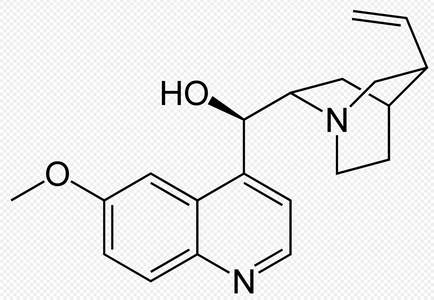
\includegraphics[scale = 0.7]{quinine.png} &
%   		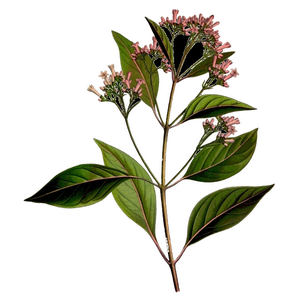
\includegraphics[scale = 0.7]{quinquina.png}\\
%   		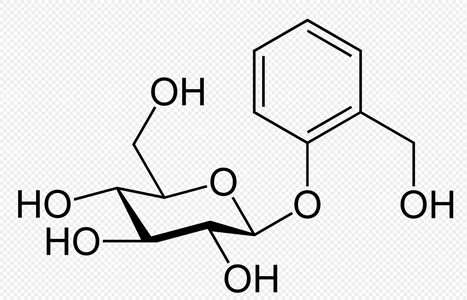
\includegraphics[scale = 0.7]{salicyline.png} &
%   		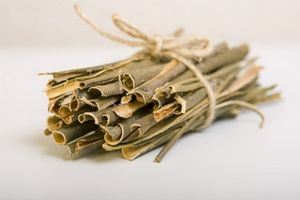
\includegraphics[scale = 0.7]{saule.png}\\
%	\end{tabular}
%	\caption{En haut, quinine et quinquina. En bas, salicyline et écorce de saule.}
%	\end{center}
%\end{figure}

\newpage
\section{Principe de la conversion}\label{sec:1}

\subsection{Rappels}

\subsubsection{Champ électromoteur}
Une charge électrique $q$ en mouvement à la vitesse $\bold{v}$ plongée dans un champ électromagnétique $(\bold{E},\bold{B})$ est soumise à la force de Lorentz :
\begin{equation}
	\bold{F} = q\left(\bold{E} + \bold{v}\times\bold{B} \right).\\
\end{equation}

Soient deux référentiels galiléens en translation rectiligne uniforme l'un par rapport à l'autre : le champ électrique n'y est pas perçu de la même manière par un observateur. Ainsi, lorsque des charges se déplacent dans un conducteur, lui-même en mouvement par rapport au référentiel du laboratoire où règne $(\bold{E},\bold{B})$, elles ressentent un champ électrique supplémentaire dépendant directement du mouvement du conducteur dans le champ magnétique : c'est le \textbf{champ électromoteur}, d'expression
\begin{equation}
	\bold{E}_m = \bold{V}\times\bold{B}.
\end{equation}

\subsubsection{Force de Laplace}

Soit le référentiel du laboratoire $\mathcal{R}$ où règne un champ $(\bold{E},\bold{B})$ : considérons un matériau conducteur en mouvement à vitesse $\bold{V}$, parcouru par un courant. La résultante des forces de Lorentz agissant sur un élément de volume $d\mathcal{V}$ de ce milieu est appelée \textbf{Force de Laplace} et elle s'écrit
\begin{equation}
	\bold{dF}_L = \rho_e d\mathcal{V}\;\bold{v}\times\bold{B} = \bold{J}\times\bold{B},
\end{equation}
où $\bold{J}$ désigne la densité volumique de courant électrique dans le conducteur (par rapport au référentiel du conducteur).

\subsection{Mise en évidence d'une conversion électromécanique de puissance}

Considérons le système des rails de Laplace : un générateur électrique est connecté à un \textbf{conducteur parfait} formé de deux rails et d'un cylindre métallique posé en travers des deux rails. Le cylindre est capable de rouler sur les rails. On place le tout dans un champ magnétique. Lorsque le courant parcourt le circuit, le barreau cylindrique mobile subit une action mécanique (la force de Laplace) qui le fait bouger dans la direction $x$.

\begin{figure}[h!]
	\begin{center}
		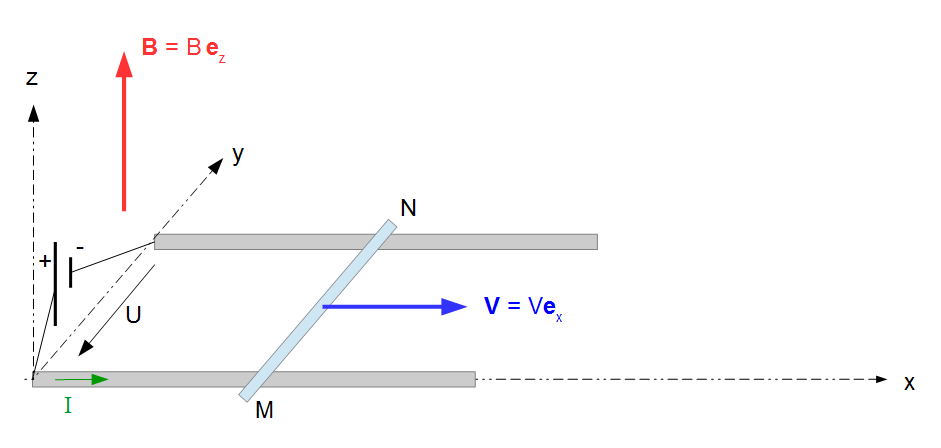
\includegraphics[scale = 0.70]{rails_Laplace.png}
		\caption{Rails de Laplace} 
		\label{fig:rails_Laplace}
	\end{center}
\end{figure}
		
Calculons la puissance de la force de Lorentz exercée sur une charge dans le barreau mobile :
\begin{equation}
	\mathcal{P} = -e\left[\left(\bold{v} + \bold{V} \right)\times\bold{B}\right]
	\cdot\left(\bold{v} + \bold{V}\right)
\end{equation}
En ne conservant que les termes non-nuls de la somme,
\begin{equation}
	\mathcal{P} = -e\left(\bold{v}\times\bold{B}\right)\cdot\bold{V} 
	-e\left(\bold{V}\times\bold{B}\right)\cdot\bold{v} = 0.
\end{equation} 

Cette puissance est nulle, mais on peut analyser chacun des deux termes de cette dernière expression :
\begin{itemize}
	\item le premier terme décrit la puissance de la résultante des forces de Laplace, responsable d'un 	mouvement du barreau mobile puisque cette force est dirigée selon l'axe $x$. Les électrons ne 			peuvent pas quitter le barreau conducteur : il y a donc un transfert de quantité de mouvement 			depuis les électrons vers le réseau cristallin, provoquant un mouvement de l'ensemble du barreau 		cylindrique. Ce terme traduit donc la \textbf{conversion d'une énergie électrique (liée à un 			courant électrique) en une énergie mécanique (liée au mouvement du conducteur)}. C'est donc une 		puissance mécanique :
	\begin{equation}
		\mathcal{P}_m \equiv -e\left(\bold{v}\times\bold{B}\right)\cdot\bold{V}; 
	\end{equation}
	
	\item le second terme décrit la puissance d'une force mécanique, liée au mouvement du barreau 			mobile, agissant sur le mouvement des électrons par rapport au circuit, donc susceptible de créer 		un courant électrique. Les électrons perçoivent en effet le terme $\bold{V}\times\bold{B}$ comme un 	champ électrique, le champ électromoteur
	\begin{equation}
		\bold{E}_m = \bold{V}\times\bold{B}.
	\end{equation}
	Ce terme est donc une puissance électrique
	\begin{equation}
		\mathcal{P}_e \equiv -e\bold{E}_m\cdot\bold{v}.
	\end{equation}
	Il s'agit donc d'une conversion d'énergie mécanique (l'énergie cinétique liée au déplacement du 		barreau mobile) en énergie électrique (la mise en mouvement des électrons sous l'effet d'un champ 		électrique correspond à la génération d'un courant électrique dans le circuit).\\
\end{itemize}

Le bilan de puissance se réécrit
\begin{equation}
	\boxed{\mathcal{P}_m + \mathcal{P}_e = 0}.
\end{equation}
\`A l'échelle du circuit, et non plus pour un seul électron
\begin{equation}
	\boxed{P_m + P_e = 0}.
\end{equation}

\subsubsection*{Modèle électrocinétique}

On peut faire une modélisation électrocinétique du système selon que c'est l'alimentation électrique (moteur, consommateur de puissance électrique) ou le mouvement du barreau conducteur (générateur, producteur de puissance électrique) qui initie le phénomène :\\
\begin{itemize}
	\item \textbf{fonctionnement en moteur :} le sens du courant délivré par l'alimentation détermine 		l'orientation du circuit ($d\ell = +dy \bold{e}_y$, donc de M vers N dans le barreau) à partir de 		laquelle on calcule la force électromotrice 
	\begin{equation}
		e = \int_M^N (\bold{V}\times\bold{B})\cdot d\ell = - VBL < 0,
	\end{equation}
	Le modèle équivalent est celui d'un générateur idéal de tension $e$ opposée à la tension 				d'alimentation $U$ (Figure \ref{ref:rail_modele} panneau de gauche.) On a donc
	\begin{equation}
		U = -e \quad\text{d'où}\quad UI = -eI = -P_e
	\end{equation}
	en multipliant par l'intensité $I$ du courant circulant dans le conducteur. Comme la force 				électromotrice est ici négative, elle a tendance à générer un courant s'opposant à I. On a alors 		plutôt tendance à définir la \textbf{force contre-électromotrice}
	\begin{equation}
		E \equiv -e > 0.
	\end{equation}	 
	Si le conducteur n'est plus parfait ($\bold{E} \neq 0$ dans tout le conducteur), on doit ajouter 		une résistance en série (Figure \ref{ref:rail_modele} panneau de droite).
	La tension aux bornes de l'ensemble s'écrit donc
	\begin{equation}
		\boxed{U = E + RI} \quad\text{et}\quad UI = EI + RI^2.
	\end{equation}
	
	On redéfinit la puissance électrique récupérée par le barreau conducteur en utilisant $E$ au lieu 		de $e$, d'où
	\begin{equation}
		\boxed{P_e \equiv EI}
	\end{equation}
	et on réécrit le bilan de puissance en conséquence :
	\begin{equation}
		\boxed{P_m = P_e}.
	\end{equation}
	
	\item \textbf{fonctionnement en générateur :} on retire l'alimentation, qu'on remplace par un 			ampèremètre et on déplace le barreau conducteur avec une vitesse $\bold{V}$ selon $\bold{e}_x$. On 		crée un champ électromoteur dirigé selon -y, donc les électrons se déplacent selon +y, donc le 			courant créé est dirigé selon -y, direction qui définit l'orientation de la f.e.m. On intègre de N 		vers M et cette fois
\end{itemize}

\begin{figure}[h!]
	\begin{center}
		\begin{tabular}{cc}
			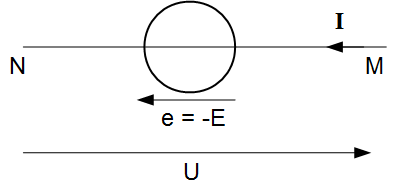
\includegraphics[scale=0.5]{rail_ideal.png} &
			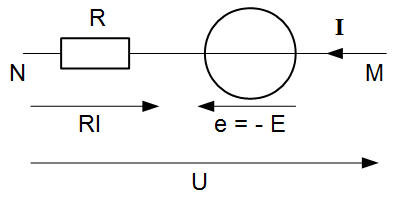
\includegraphics[scale=0.5]{rail_reel.png} \\
		\end{tabular}
	\end{center}
	\caption{Gauche : moteur idéal ; Droite : moteur avec résistance interne}
	\label{ref:rail_modele}
\end{figure}

Nous venons d'illustrer le principe de la conversion électromécanique de puissance à travers l'exemple du rail de Laplace. Ce système produit un mouvement de translation en convertissant de l'énergie électrique en énergie mécanique : c'est le principe de fonctionnement d'un moteur linéaire. Comment faire pour obtenir un mouvement de rotation ?

\subsection{Machine tournante}

\textcolor{blue}{Voir feuille annexe : Couple moteur sur une spire carrée dans un champ magnétique uniforme.}\\

\textit{Remarque : cette spire carrée est une boucle de courant, de moment magnétique $\mathcal{M} = -IS \bold{e}_x$. Le couple des forces résultant de l'action de $\bold{B}_0$ sur le courant $i$ vaut donc}
\begin{equation}
	\bold{C} = \mathcal{M}\times\bold{B}_0 = ISB_0 (-\bold{e}_x \times \bold{e}_z) = ISB_0 \bold{e}_y
	= IB_0 DL \bold{e}_y.
\end{equation}
On retrouve le résultat calculé "mécaniquement". La grandeur $B_0 DL$ est homogène au flux du champ magnétique $\Phi_0$ à travers la spire lorsque le champ est perpendiculaire au plan de la spire. On écrit donc
\begin{equation}
	\boxed{C = I \Phi_0}.
\end{equation}
On peut donc générer un mouvement de rotation : nous venons de décrire, de façon très simplifiée, le principe de fonctionnement d'un moteur. Notons qu'on peut faire comme pour le moteur linéaire : remplacer l'alimentation par un ampèremètre et forcer mécaniquement la rotation du moteur pour générer un courant électrique. Ce type de machine peut donc être utilisé comme moteur ou comme générateur.

\newpage
\section{Machine à courant continu}\label{sec:2}

La machine a courant continu est historiquement la première a avoir été inventée.

\subsection{Structure du moteur}

Définissons les principaux éléments de ce moteur : \\
\begin{itemize}
	\item \textbf{Circuits magnétiques :}
	\begin{itemize}
		\item Le stator est la partie fixe du moteur, portant le circuit inducteur.
		\item Le rotor est la partie mobile, reliée à l'arbre moteur, sur laquelle est bobiné le 				circuit induit.
	\end{itemize}
	\item \textbf{Circuits électriques :}
	\begin{itemize}
		\item L'inducteur : constitue la source de champ magnétique dans la machine. Il est réalisé 			soit à partir d'aimants permanents (machines de faible puissance, en robotique par exemple), 			soit à l'aide d'un électro-aimant;
		\item L'induit : circuit électrique soumis au champ magnétique produit au niveau du stator et 			placé sur le rotor;
	\end{itemize}
\end{itemize}

La machine à courant continu comporte deux bobinages, l'un porté par le stator et l'autre par
le rotor. Le stator et le rotor, constitués d'un matériau magnétique à base de fer, sont séparés par
un entrefer. Il doit être suffisamment faible pour optimiser le couplage entre le champ généré au stator et l'induit, ce qui permet de limiter la consommation de l'inducteur. L'ensemble forme un circuit magnétique où les lignes de champ traversant l'entrefer et le rotor se referment dans le stator.

\subsubsection*{Circuit statorique}

Deux bobinages identiques portés par les deux cols situés de part et d'autre du rotor sont connectés
en série et donc parcourus par le même courant inducteur permanent de d'intensité $I_e$. Le champ magnétique créé par l'inducteur est donc permanent.\\ 

\textit{En négligeant les effets de bord, les plans orthogonaux à l'axe de rotation, tel que le plan de coupe étudié, sont des plans d'antisymétrie de la distribution de courant inducteur. Par conséquent, les lignes de champ magnétique sont contenues dans ce plan. La simulation numérique des équations locales satisfaites par le champ magnétique permet de simuler la géométrie de ces lignes de champ. L'entrefer étant entouré de deux cylindres en matériau de perméabilité magnétique infinie, les lignes de champ dans l'entrefer, orthogonales aux cylindres, sont radiales.}

\begin{figure}[h!]
	\begin{center}
	\begin{tabular}{cc}
		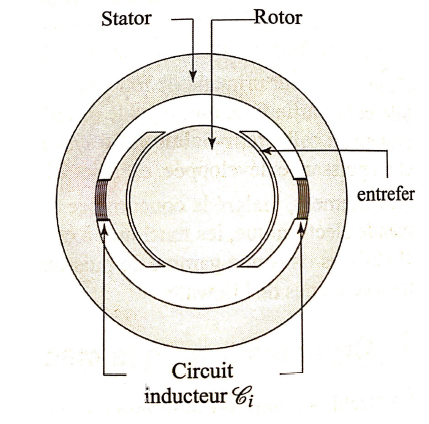
\includegraphics[scale = 0.60]{mcc_principe.png} &
		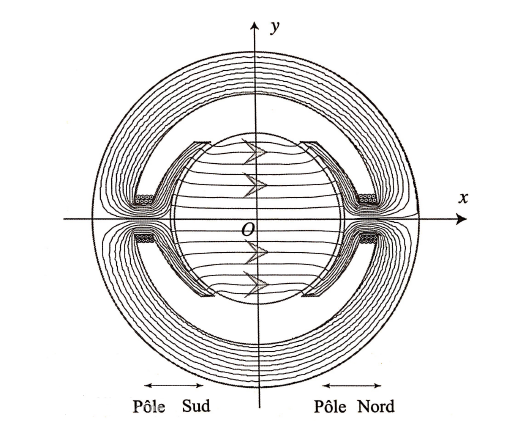
\includegraphics[scale = 0.60]{mcc_fieldlines.png}\\
	\end{tabular}
	\end{center}
	\caption{Gauche : stator, rotor, inducteur ; 
	Droite : lignes de champ dans le circuit magnétique.} 
	\label{fig:rails_Laplace}	
\end{figure}
		
\subsubsection*{Circuit rotorique}

Le rotor est constitué d'un enroulement de spires conductrices, réunies en faisceaux et positionnées dans les encoches de la structure, de telle sorte que lorsqu'un côté de l'enroulement fait face au pôle nord, l'autre est au pôle sud (on retrouve alors la configuration traitée dans la dernière partie du grand un : une spire rectangulaire, plongée dans le champ magnétique produit par le stator).

\begin{figure}[h!]
	\begin{center}
		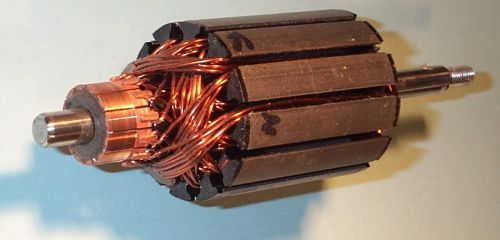
\includegraphics[scale = 0.60]{rotor.png}
	\end{center}
	\caption{Rotor.} 
	\label{fig:rails_Laplace}	
\end{figure}

Ces spires sont parcourues par un courant d'intensité I fourni par une alimentation électrique extérieure. Comme le courant électrique provient généralement d'une source extérieure fixe, et donc pour ne pas emmêler les fils durant la rotation, les bobines du rotor sont alimentées par des \textbf{contacts électriques frottants}, entre d'une part :
\begin{itemize}
	\item les \textbf{balais} (ou charbons) fixés sur le stator, et d'autre part
	\item le \textbf{collecteur}, fixé sur le rotor.
\end{itemize}
Le collecteur a une autre utilité : il permet d'inverser le sens du courant. Les forces font tourner la spire autour de l'axe de rotation du moteur, mais quand la spire a fait un demi-tour, il est faut inverser le sens du courant pour continuer le mouvement. Ce système est sujet à l'usure et nécessite un entretien régulier. Il implique également une limitation en vitesse de rotation.

\subsubsection*{Couple électromagnétique, couple résistant}

On va supposer que le moteur est un \textbf{moteur à excitation indépendante} : les circuits de l'inducteur et de l'induit sont indépendants électriquement (on parle aussi de moteur à flux constant). La grandeur mécanique d'intérêt est le couple de forces de Laplace exercé sur le rotor. Nous avons calculé ce \textbf{couple électromagnétique} pour une spire dans la section précédente :
\begin{equation}
	C = \Phi_0 I.
\end{equation}
Lorsque le flux $\Phi_0$ est constant (ce qui est le cas car le circuit inducteur travaille à flux constant : aimants permanents, ou électroaimant dont le bobinage est traversé par un courant constant), le couple électromagnétique est proportionnel au courant d'alimentation $I$ de l'induit.\\

La puissance mécanique associée à ce couple s'écrit
\begin{equation}
	P_m = C\Omega
\end{equation}
si $\Omega$ est la vitesse angulaire (en rad/s) de l'arbre-moteur.\\ 

Soit J le moment d'inertie du rotor par rapport à l'axe de l'arbre-moteur. Le théorème du moment cinétique appliqué au rotor s'écrit alors
\begin{equation}
	J\frac{d\Omega}{dt} = C - C_r - f\Omega,
\end{equation}
où $-f\Omega$ désigne une force de frottement fluide et $C_r$ le couple résistant exercé par la charge entraînée par le moteur (si $C_r = 0$ on dit que le moteur fonctionne à vide). En régime permanent et si les frottements sont négligeables, on a
\begin{equation}
	C = C_r.
\end{equation}
Cette condition donne le \textbf{point de fonctionnement} de la machine en régime permanent.\\

\textbf{En régime permanent, c'est donc la charge mécanique du moteur (le milieu extérieur responsable du couple résistant) qui impose le couple électromagnétique à fournir pour l'entraîner à vitesse de rotation constante, et par conséquent la valeur courant $I$ circulant dans l'induit à fournir pour produire le couple $C = C_r$.}
 
\subsection{Modèle électrocinétique de l'induit}

Comme dans le problème des rails de Laplace, il s'établit dans l'induit une force contre-électromotrice (ou force électromotrice en convention électrotechnique) E. Pour la déterminer, on part du bilan de puissance
\begin{equation}
	P_m = P_e \quad\text{d'où}\quad C\Omega = EI.
\end{equation}
On injecte dans $C$ son expression en fonction de $I$, d'où
\begin{equation}
	\boxed{E = \Phi_0 \Omega}.
\end{equation}
Ici, $\Phi_0$ joue le rôle de \textbf{constante de force électromotrice}.\\

En régime établi, le circuit induit d'un MCC à excitation indépendante peut être représenté par l'association d'une résistance $R$ (résistance de l'induit) et d'un générateur de tension de force électromotrice $E$, dirigée selon la tension aux bornes de l'induit $U$ :
\begin{equation}
	U = E + R I
\end{equation}

Si on néglige la chute de tension résistive dans l'induit, on voit qu'il existe une relation de proportionnalité entre la tension d'alimentation de l'induit $U$ et la vitesse de rotation du moteur $\Omega$, ce qui rend un tel moteur très simple à commander. C'est cette simplicité de commande qui a justifié l'intérêt de cette machine, qui a longtemps été la seule pour laquelle c'était aussi simple.\\ 

\begin{figure}[h!]
	\begin{center}
		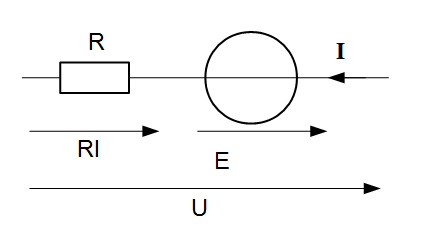
\includegraphics[scale=0.5]{mcc_modele.png}
	\end{center}
	\caption{Modèle électrocinétique de l'induit du moteur à courant continu 
	à excitation indépendante.}
	\label{ref:mcc_modele}
\end{figure}

En convention récepteur (celle choisie pour représenter le modèle), le sens des flèches de $I$ et $E$ indiqués sur le schéma correspondent à des valeurs de $I$ et $E$ positives. Dans cette convention, lorsque
\begin{itemize}
	\item $E > 0$ et $I >0$, la puissance électrique $P_e = EI > 0$ : la machine reçoit de la puissance 	électrique et fournit de la puissance mécanique. Elle fonctionne en moteur;
	\item la machine fonctionne en générateur si $EI < 0$ (en convention récepteur) : elle reçoit de la 	puissance mécanique et fournit de la puissance électrique.\\
\end{itemize}

\begin{figure}[h!]
	\begin{center}
		\begin{tabular}{cc}
			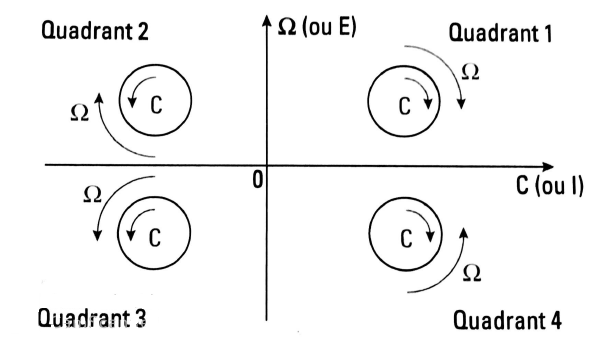
\includegraphics[scale=0.5]{quadrants.png} &
			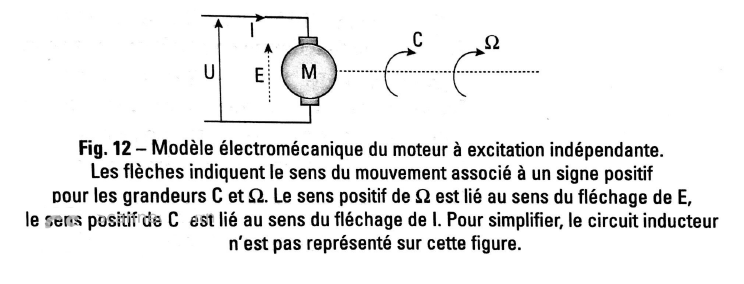
\includegraphics[scale=0.5]{conventions.png} \\
		\end{tabular}
	\end{center}
\end{figure}

On peut représenter les régimes de fonctionnement de la machine à courant continu dans un diagramme $(\Omega, C)$ : on obtient les quatre quadrants de la machine à courant continu :
\begin{itemize}
	\item Quadrant 1 : $EI > 0$ avec $E > 0$ (donc  $\Omega > 0$) et $I > 0$. 
		Fonctionnement moteur, l'arbre tourne dans le sens choisi positif
	\item Quadrant 2 : $EI < 0$ avec $E > 0$ et $I < 0$. 
		Fonctionnement en générateur et tourne dans le sens positif.
	\item Quadrant 3 : $EI > 0$ avec $E < 0$ et $I < 0$. 
	Fonctionne en moteur et tourne dans le sens négatif.
	\item Quadrant 4 : $EI < 0$ avec $E < 0$ et $I > 0$. 
	Fonctionne en générateur et tourne dans le sens négatif.
\end{itemize}

\subsubsection*{Emballement de la machine}

p135 Bréal, électrotechnique et conversion de puissance (PSI)

\subsection{Bilan de puissance}

p135 à 137, idem.

\textcolor{blue}{Manip...}
                                                                                                                                                                                                                                   
\subsection{Fonctionnement en régime variable}

\subsubsection{Modèle électrocinétique}
p133
\begin{figure}[h!]
	\begin{center}
		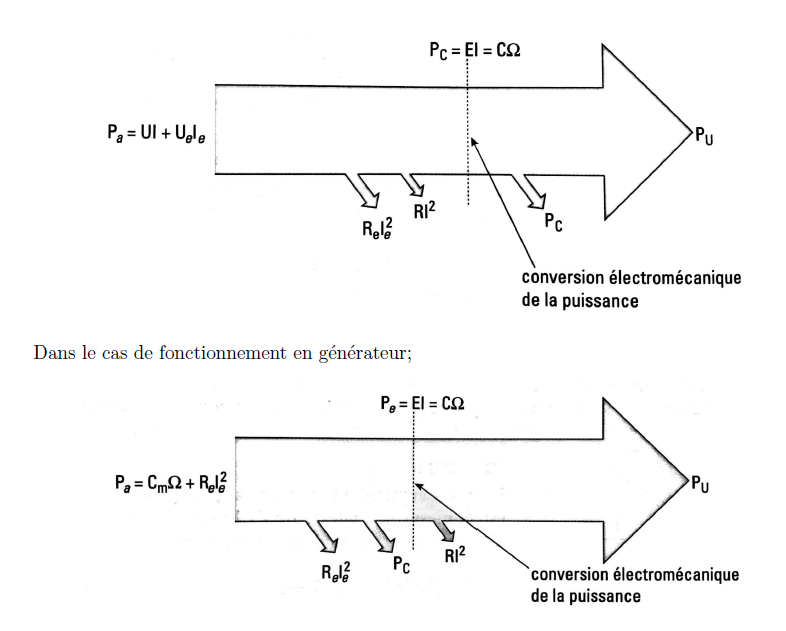
\includegraphics[scale = 0.50]{bilan_puissance.png}
		\caption{Bilan de puissance. Haut : moteur. Bas : générateur.} 
		\label{fig:rails_Laplace}
	\end{center}
\end{figure}

\subsubsection{Schéma fonctionnel}
p138-139

\begin{figure}[h!]
	\begin{center}
		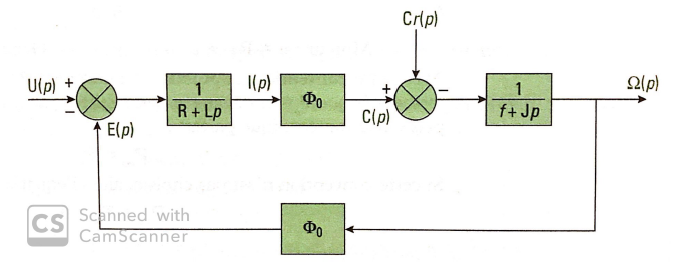
\includegraphics[scale = 0.70]{aservissement.png}
		\caption{Rails de Laplace} 
		\label{fig:rails_Laplace}
	\end{center}
\end{figure}

\newpage
\section*{Conclusion}

L'asservissement de la vitesse de rotation des moteurs à courant continu a été maîtrisé bien avant ceux pour les autres types de moteur. Ils ont donc longtemps été appréciés pour cette facilité de commande. Néanmoins, à puissance égale, les moteurs à courant continu sont beaucoup plus coûteux que les moteurs
asynchrones : bobinages au stator et au rotor, collecteur, balais, maintenance importante. Le système balais-collecteur est fragile et nécessite une surveillance et un entretien fréquent. Par exemple, les moteurs TGV Paris-Sud-Est doivent subir un démontage complet tous les 300000 km, soit environ une fois par an. On leur préfère donc, dès que c'est possible, des moteurs à courant alternatif. Ils restent très utilisés dans le domaine de l'automobile : démarreur, pompe à carburant, essuie-glace, ouverture des vitres, climatiseur...

Ouverture vers les moteurs synchrone et asynchrone. Rapidement, principe de fonctionnement et applications :
\begin{itemize}
	\item moteur synchrone
	\item moteur asynchrone
\end{itemize}
\newpage
\section*{Annexes}

\end{document}